\chapter{Implementación sobre Qanus}
\label{chap:qanus} \label{chap:5}
\faltadependiente
En este capitulo veremos la implementación del modelo de question answering multilingüe y diferentes evaluaciones realizadas utilizando como guia dos tareas monolingües de la competencia QA@Clef '07, una para español y otra para portugués. El sistema está basado en un framework académico de código abierto llamado Qanus. Este framework está empaquetado con una sistema de QA simple, QA-sys, que resuelve ejercicios de la competencia Trec '07 con soporte para inglés. Nosotros adaptamos este sistema para utilizar como librería de procesamiento de lenguajes a Freeling, generando un sistema baseline multilingüe. A este sistema le agregamos features reseñados en \allref{sec:literatura} y realizamos diferente mediciones sobre las instancias en español y portugués sobre los ya mencionados ejercicios de Clef '07.

La estructura de este capitulo es la siguiente: en \allref{sec:ejecicio-de-clef} se describe con detalle el panorama general de tareas de question answering en la competencia Clef '07, haciendo énfasis en las tareas seleccionadas, en los corpus y las preguntas disponibles y en las decisiones tomadas a la hora de elegir estas tareas; en \allref{sec:sistema} se comenta la adaptación del sistema baseline y las modificaciones realizadas a los algoritmos, {\color{red}mientras que los resultados pueden observarse como apartados en las mismas secciones o como una sección aparte al final}.

\section{Ejercicio de Clef}
\label{sec:ejecicio-de-clef}
Tras investigar distintas competencias y métodos de evaluación, optamos por utilizar como guía de trabajo dos ejercicios de la tarea principal de question answering de la competencia Clef de 2007. Principalmente por contar con un subconjunto de ejercicios bastante adecuados para nuestra tesis y disponer de un corpus de datos libre y disponible en el acto para evaluar una parte importante de las funcionalidades implementadas en nuestro proyecto. 

Como mencionamos en \allref{subsec:competencias}, Clef (de \textit{Cross-Language Evaluation Forum}) es una organización que busca fomentar la investigación en sistemas de information retrieval cross-language. En particular, una vez por año Clef lanza una competencia de Question Answering multilingüe, con diferentes corpus y diferentes tipos de ejercicios. Estas competencia permiten obtener un patrón estándar de comparación entre distintos desarrollos y una idea general del estado de arte alcanzado en los diferentes idiomas por la diferentes actores académicos y comerciales. Por lo demás, Clef es el principal organizador de conferencias de question answering multilingüe para idiomas europeos y la tarea principal de '07 presentaba una complejidad adecuada para el scope de esta tesis.

La competencia de 2007 es la quinta campaña de QA multilingüe de Clef, siendo la primera en 2003.

La tarea estandar principal de question answering incorpora algunas particularidades que la diferencian de anteriores campañas: los temas o tópicos, la co-referencia y el uso de wikipedia como corpus de datos parcial. Además de la tarea principal se presentaron tres tareas más: Answer Validation Exercise (AVE) y QUAST, question answering in speech transcription y Question Answering Real Time, con métricas de performance temporales. Como nota general, es importante notar que las tareas fueron de una complejidad elevada y en comparación con los resultados del año anterior, la mejor precisión general bajó del 49\% al 41.75\% para tareas multi-lingües, mientras que, más significativamente, bajó de 68\% a 54\% en tareas monolingües.


\subsection{Tareas}
\label{subsec:tareas}
Utilizamos como guia dos ejercicios de la tarea principal de question answering de '07  por varias razones (Ver \cite{GuidelineClef07} y \cite{OverviewClef07} para un detalle exhaustivo de la conferencia en cuestión). Para esta tarea estaban disponibles en acto corpus, inputs de prueba y resultados esperados para una experimentación multilingüe que abarque tanto inglés como español y portugués. Además, estos ejercicios incorporaban, por única vez, diferentes wikipedias como parte del corpus de datos, lo cual resulta de por si atractivo. 

La tarea principal de QA de Clef '07 ofrece dos grandes grupos de ejercicios:
\begin{itemize}
\item Mono-lingual: donde el idioma de la pregunta y el idioma de la fuente de información son el mismo
\item Cross-lingual: donde el idioma de la pregunta y el idioma de la fuente de información difieren
\end{itemize}

En ambos grupos, los sistemas reciben un set de 200 preguntas - que pueden ser de hechos o eventos (factoid), definiciones de personas, cosas u organizaciones (definition), listas de personas, objetos o datos (list) - y se exige devolver una respuesta exacta, donde exacta significa sin más información de la mínima necesaria. Siguiendo el ejemplo de Trec, los ejercicios de este año contienen topics, i.e. clusters de preguntas relacionadas con un mismo tema y con posibilidad de co-referencia entre las preguntas del grupo. Ni el tipo de la pregunta ni el tópico es dado a los participantes.

La respuesta tiene que estar soportada por el id del documento del cual se extrajo y por la porción de texto que proveyó contexto suficiente para soportar la corrección de la respuesta. Los “textos de soporte” pueden venir de diferentes partes de documentos relevantes y deben sumar un máximo de 700 bytes. No hubo restricciones sobre la longitud del string de respuesta, pero fragmentos de información innecesaria fueron penalizados marcando la respuesta como ineXacta. 

Otra particularidad de los ejercicios es que hay preguntas sin respuesta en el corpus que esperan como respuesta 'Nil'.


Se consideraron 10 idiomas para preguntas: búlgaro, holandés, inglés, francés, alemán, indonesio, italiano, portugués, romano y español. Todos estos idiomas se usaron como idiomas del corpus, a excepción del indonesio para el que no se disponía de una colección de noticias.

Se propusieron, en total, 37 tareas concretas: 8 monolingües y 29 bilingües. Dada la complejidad de la construcción del ejercicio mismo, la organización solo implementó concretamente las tareas tomadas por algún equipo competidor. 


\begin{figure}
  \centering
    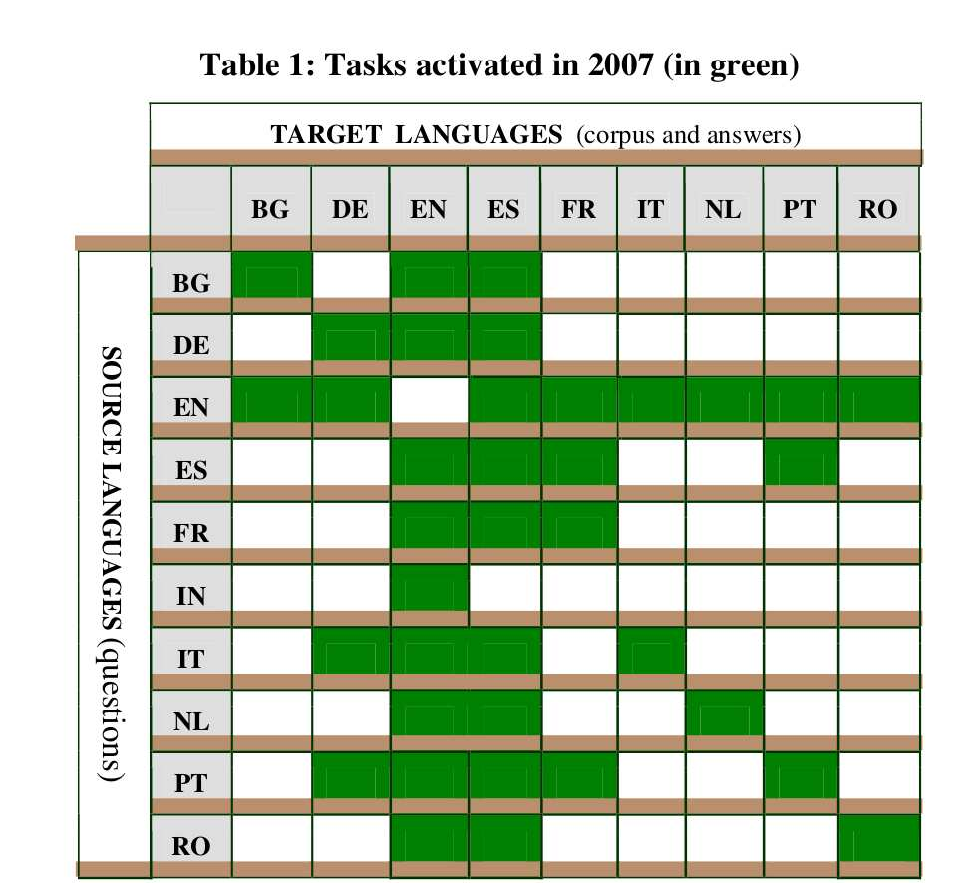
\includegraphics[scale=0.5]{graficos/clef07}
  \caption{Tareas activadas en la competencia Clef '07}
  \label{fig:tareas}
\end{figure}

El corpus de datos propuesto consiste en dos corpora distintos: una serie de de recopilados especificamente por los organizadores de la competencia y utilizado con frecuencia en competencias anteriores y, por otro lado, snapshops de las wikipedias en diferentes idiomas con límite en Diciembre de 2006.

Para nuestro proyecto utilizamos las preguntas y los datos de evaluación de los ejercicios monolingües es-es (español-español) y pt-pt (portugués-portugués) implementando como corpus de datos solo las wikipedias.

Los datos de los ejercicios constan de dos archivos: un archivo con 200 preguntas agrupadas por temas y otro archivo con diferentes traducciones de la pregunta, una respuesta goldstandard con soporte textual y el id del documento de soporte para el idioma target (del corpus). 

Por otro lado, en la guía de ingreso a la competencia\cite{GuidelineClef07} se proveen links para descargar los snapshots de wikipedia sugeridos. Se ofrece una versión de wikipedia en inglés preprocesada de Noviembre de 2006 \footnote{\url{http://ilps.science.uva.nl/WikiXML/}}, dos opciones para descargar wikipedia en español: una imagen estática en html de Noviembre de 2006 \footnote{\url{http://static.wikipedia.org/downloads/November_2006/es/}} y un dump xml de Diciembre de 2006 \footnote{\url{http://download.wikimedia.org/images/archive/eswiki/20061202/pages-articles.xml.bz2}} y también X opciones de portugués.

La guía aclara que, bajo responsabilidad de los participantes, se puede usar
cualquier otra versión de Wikipedia, siempre y cuando sea anterior a noviembre / diciembre de 2006.
Además, se pide que las respuestas sean tomadas de ``entradas reales" o artículos de wikipedia y
no de otros documentos (imagenes, discusión, categoría, template, histórico de reviosones, datos de usuario y páginas con meta información).

Los links a páginas de wikipedia en español y en portugués no estaban más disponibles (ambos respondieron 404), mientras que el formato
preprocesado pedido para el inglés resultaba realmente complejo de instalar y parecía una linea muerta. Por estos motivos,
seguimos la sugerencia sobre el uso responsable de otras wikipedias y utilizamos las siguientes snapshots de Wikidumps\footnote{Ver \url{http://dumps.wikimedia.org/} y \url{http://en.wikipedia.org/wiki/Wikipedia:Database_download\#Other_languages}}.

\begin{center}
\begin{tabular}{ | l | l | l | l |}
    \hline
    Idioma & Fecha & Tamaño & \# Entradas \\ \hline
    Español & 5 de Julio de 2006 & 558M  & 233750  \\ \hline
    Portugués & 1 de Febrero de 2007 & 776M  & 498039  \\ \hline
    Inglés Simple & 4 de Julio de 2006 & 26M   & 18273   \\ \hline
    Inglés & 4 de Noviembre de 2006 & 7,6G  &   \\ \hline
    Español & 26 de Enero de 2007 & 902M  &   \\ \hline
    Español & 14 de Junio de 2013 & 7,3G  &   \\ \hline
    Inglés Simple & 24 de Julio de 2013 & 406M  &   \\ \hline
\end{tabular}  
\end{center}

Utilizando la información disponible en los archivos de respuestas esperadas, discriminamos las preguntas con respuestas con soporte de wikipedia, las soportadas por el corpora de noticias de la organización y las que no tienen respuesta (NIL):

\begin{center}
\begin{tabular}{| l | l | l | l | l |}
\hline
Idioma & Wiki & News & NIL & Total \\ \hline
es & 155 & 37 & 8 & 200 \\ \hline
pt & 130 & 59 & 11 & 200 \\ \hline
\end{tabular}
\end{center}


\subsection{Análisis de las preguntas}

Las 200 preguntas del test set están agrupadas por tema, y cada tema tiene de una a cuatro preguntas. Los temas pueden ser entidades nombradas, evento o también categorías como objetos, fenómenos naturales, etc (por ejemplo: Bush, Juegos Olímpicos, notebooks, huracanes, etc). 
Los temas no están dados en el set de test, pero pueden ser inferidos del primer par pregunta respuesta. La relación del tema con el grupo de preguntas respetaba las siguiente condiciones:

\begin{itemize}
\item El tema es nombrado en la primer pregunta o bien en la primera respuesta.
\item Las siguientes preguntas pueden contener co-referencias al tema expresado en el primer par pregunta/respuesta
\end{itemize}


Para ilustrar el punto consideremos el primer grupo de preguntas para el ejercicio de español es:
\begin{itemize}
\item ¿En qué colegio estudia Harry Potter?
\item ¿Cuál es el lema del colegio?
\item ¿En qué casas está dividido?
\item ¿Quién es el director del colegio?
\end{itemize}


Como ya mencionamos, algunas preguntas podían no tener respuesta en la colección de documentos, y en ese caso la respuesta exacta era “NIL” y la justificación y el docid vacíos. La organización definió como criterio de inexistencia de la respuesta que ni los asesores humanos ni los demás sistemas participantes pudieran encontrar alguna.

En lo que respecta a los tipos de pregunta, el ejercicio considerara tres categorías: Factoid, Definition y Closed List.

\begin{center}
\begin{table}
\begin{tabular}{| l |  p {12cm} |}
\hline
Tipo & Descripción  \\ \hline
FACTOID & preguntas fácticas, preguntando el nombre de una persona, un lugar, la medida de algo, el día en que algo ocurrió, etc. \\ \hline
DEFINITION & preguntas como Qué/ Quién es X? \\ \hline
CLOSED LIST & questions that require one answer containing a determined number of items, e.g \\ \hline
\end{tabular}
\caption{Definición de los tipos de pregunta}
\label{table:question-type-definition}
\end{table}
\end{center}

Todos los tipos de pregunta podian contener restricciones temporales, i. e: una especificación temporal proveyendo importante información para devolver una respuesta correcta. Por ejemplo: \newline
Q: Who was the Chancellor of Germany from 1974 to 1982? \newline
A: Helmut Schmidt.\newline
Q: Which book was published by George Orwell in 1945?\newline
A: Animal Farm.\newline
Q: Which organization did Shimon Perez chair after Isaac Rabin’s death?\newline
A: Labour Party Central Committee.\newline


%Los calculos propios coinciden con el análisis presentado en \cite{OverviewClef07} en la siguiente discriminación del total de preguntas en función de las categorías recién señaladas:
\begin{center}
\begin{table}[H]
\centering
\begin{tabular}{| l | l | l | l | l | l |}
\hline
Subset & Idioma & Factoid & Definition & List & Total \\ \hline
\multirow{2}{*}{Todo} & es & 158 & 32 & 10 & 200 \\ \cline{2-6}
 & pt & 159 & 31 & 10 & 200 \\ \hline
 \multirow{2}{*}{Wiki} & es & 122 & 24 & 9 & 155 \\ \cline{2-6}
 & pt & 104 & 18 & 8 & 130 \\ \hline
\end{tabular}
\caption{Totales por tipo de pregunta}
\label{table:totals-type-question}
\end{table}
\end{center}

Los tipos de preguntas disponen a su vez de subtipos. Las preguntas factoid disponen de 8 subtipos, las de definiciones y listas tienen 4.
Se consideraron los siguiente 8 tipos de Factoids: 

\begin{center}
\begin{table}[H]
\centering
\begin{tabular}{| l | p{12cm}|}
\hline
Tipo & Ejemplo \\ \hline
PERSON &  Q: Who was called the \dq{Iron-Chancellor}? \newline A: Otto von Bismarck. \\ \hline 
LOCATION & Q: Which town was Wolfgang Amadeus Mozart born in? \newline A: Salzburg. \\ \hline
ORGANIZATION & Q: What party does Tony Blair belong to? \newline A: Labour Party.\\ \hline
MEASURE &Q: How high is Kanchenjunga?\newline A: 8598m. \\ \hline
COUNT & Q: How many people died during the Terror of Pol Pot? \newline A: 1 million.\\ \hline
OBJECT & Q What does magma consist of?\newline A: Molten rock.\\ \hline
TIME & Q: What year was Martin Luther King murdered?\newline A: 1968.\\ \hline
OTHER & i.e. todo lo que no encaja en las categorías anteriores.\newline Q: Which treaty was signed in 1979? \newline
A: Israel-Egyptian peace treaty.\\ \hline
\end{tabular}
\caption{Tipos de respuesta esperada para preguntas Factoid}
\label{table:type-factoid}
\end{table}
\end{center}

Las preguntas de tipo LIST consisten son enumeraciones de 4 tipos posibles: PERSON, LOCATION, ORGANIZATION y OTHER.
Por ejemplo:\newline
Q: Name all the airports in London, England. \newline
A: Gatwick, Stansted, Heathrow, Luton and City.

Como solo una fuente estaba estaba permitida, los items debían aparecer en secuencia, uno después del otro, en uno documento de la colección .
Con respecto a las preguntas de tipo definition, también cuatro tipos, con otra semántica.


\begin{center}
\begin{table}[H]
\centering
\begin{tabular}{| l | p{12cm}|}
\hline
Tipo & Descripción y ejemplo \\ \hline
PERSON & i.e. preguntas sobre el rol, el trabajo o información importante de alguien \newline
 Q: Who is Robert Altmann? \newline
 A: Film maker. \\ \hline
ORGANIZATION & i.e. preguntas sobre la misión, el nombre completo o información relevante sobre una organización \newline
 Q: What is the Knesset? \newline
 A: Parliament of Israel. \\ \hline
OBJECT & i.e. preguntas por la descripción o función de objetos \newline
Q: What is Atlantis? \newline
A: Space Shuttle. \\ \hline
OTHER & i.e. preguntas por descripciones de fenómenos naturales, tecnologías, procedimientos legales, etc. \newline
Q: What is Eurovision? \newline
A: Song contest. \\ \hline
\end{tabular}
\caption{Tipos de respuesta esperada para preguntas Definition}
\label{table:definition-questions}
\end{table}
\end{center}

\begin{center}
\begin{table}[H]
\centering
\begin{tabular}{| l | l | l | l | l | l |l |l|l|}
\hline
Tipo & pt & es & pt-factoid & es-factoid & pt-def & es-def & pt-list & es-list \\ \hline
COUNT & 21 & 22 & 21 & 22 & 0 & 0 & 0  & 0\\ \hline
OBJECT & 11 & 27 & 6  & 18 & 5 & 9 & 0  & 0\\ \hline
MEASURE & 15 & 20 & 15 & 20 & 0 & 0 & 0  & 0\\ \hline
PERSON & 33  & 35 & 21 & 24 & 9 & 8 & 3 & 3\\ \hline
TIME & 19 & 16 & 18 & 16 & 0 & 0 & 1 & 0\\ \hline
LOCATION & 33 & 18  & 30 & 18 & 0 & 0 & 3 & 0 \\ \hline
ORGANIZATION & 31 & 32 & 24 & 22 & 6 & 8 & 1 & 2\\ \hline
OTHER & 37 & 30 & 24 & 18 & 11 & 7 & 2 & 5 \\ \hline
Total & 200 & 200 & 159 & 158 & 31 & 32  & 10 & 10\\ \hline
\end{tabular}
\caption{Tipos de respuesta esperada en función de tipo de pregunta}
\label{table:tipo-general}
\end{table}
\end{center}


\section{Sistema}
\label{sec:sistema}

Nuestra implementación está basada en Qanus como framework o arquitectura de diseño de QA y en Freeling como proveedor de servicios de procesamiento de lenguaje multilingue. Qanus (Question-Answering @ National University of Singapore) es un framework de question answering basado en information retrieval y también un sistema de QA funcional simple construido sobre este framework. El proyecto se actualizó por última vez en noviembre de 2012 y contiene herramientas actuales de nlp para inglés (el POS-tagger, el NER-tagger y el Question Classifier de Stanford) y también de information retrieval (índice de búsquedas lucene) bajo licencia de código abierto. El paquete cuenta con un framework (qanus), que cumple un rol equivalente a la arquitectura DeepQA en la organización del proyecto de IBM, y un sistema montado sobre este framework -QA-sys-, equivalente a Watson (Ver Figura ~\ref{fig:Quanus}). 


\begin{figure}
  \centering
    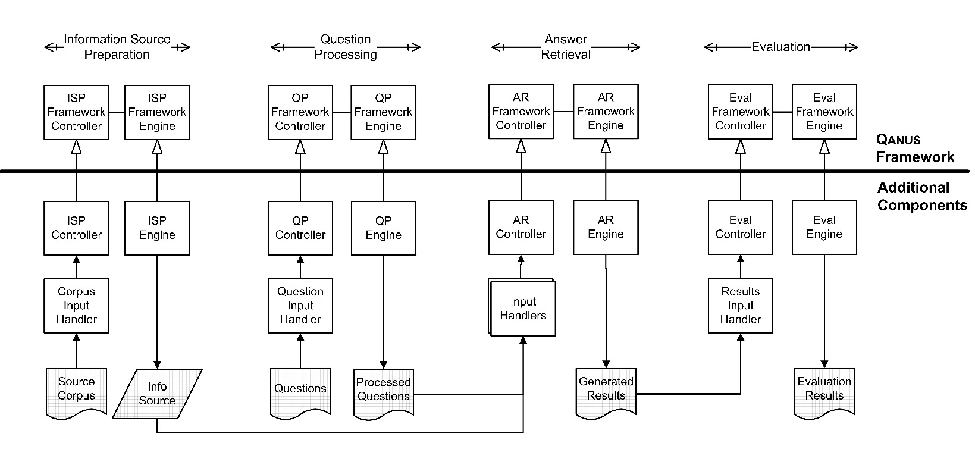
\includegraphics{graficos/Quanus}
  \caption{El framework Quanus y la implementación QA-sys}
  \label{fig:Quanus}
\end{figure}


La arquitectura de Qanus mantiene la estructura de pipeline típica similar a las reseñadas en la sección \allref{chap:estado-de-arte}. 
Consta de los siguientes pasos: \newline

\textbf{Preparación de la fuente de información: } El primer step del pipeline es preprocesar las fuentes de información para un acceso optimizado en pasos posteriores del proceso. La implementación QA-sys incorpora una base de conocimiento en formato XML de aquaint a un índice de
búsquedas Lucene. En este paso se incorpora todo el conocimiento offline; bases de conocimiento dinámicas como la web se modelan en el pasos posteriores. \newline

\textbf{Análisis de la pregunta: } Este paso, igualmente genérico, permite la incorporación de
distintos componentes para anotar los tokens de la pregunta con datos
útiles para ser consumidos por el paso 3. Otro procesamiento a
realizar en este paso podría ser la generación de queries
entendibles por los distintos motores de almacenamientos de
información del paso 1. En particular, la implementación trae un
pos-tagger, un ner-tagger y un question classiffier, todos de Stanford.
Hablaremos más de estos componentes más adelante. \newline

\textbf{Generación de respuestas: } En este paso se utiliza la información generada en la preparación
de la base de información y en el procesamiento de la pregunta para
generar una respuesta. También puede incorporarse accesos a la web y
validaciones de las respuestas candidatas. La implementación concreta
evalúa cada pasaje de los primeros n documentos retornados por Lucene
para la pregunta original con una serie de componentes ad-hoc de
distancia para adjudicar diferentes grados de confiabilidad a los
distintos pasajes. \newline


Además, se provee de un cuarto paso opcional (el sistema de QA está
completo con los tres pasos anteriores), para la fase de desarrollo y
de evaluación de la performance del sistema:\newline


\textbf{Evaluación: }Este paso está pensado para evaluar las respuestas generadas y
presentarlas de un modo conciso en la fase de desarrollo.
Básicamente, cruza las respuestas obtenidas contra unas respuestas
esperadas escritas a mano y presenta el total de respuestas dadas
correctamente.\newline

En esta sección de la tesis adoptamos el framework Qanus y adaptamos el sistema QA-sys para 1) incorporar Freeling como librería de herramientas de procesamiento del lenguaje permitiendo un funcionamiento multilenguaje, 2) trabajar sobre el corpus de datos y preguntas de los ejercicios de CLEF '07 de español y portugués descriptos en \allref{sec:ejecicio-de-clef} y, finalmente, 3) incorporamos y evaluamos diferentes mejoras tomadas de la reseña a la literatura científica del apartado anterior \allref{sec:literatura}.

\subsection{Implementación de Qanus y QA-sys}

El código está escrito en java y mantiene una interfaz común a
todos los pasos: un controller cuyas responsabilidades son cargar los
componentes y un engine que utiliza los componentes para leer el input,
procesarlo y grabar el resultado. La adaptabilidad del framework está
dada en la posibilidad de incorporar componentes respetando la interfaz
especificada para los mismos o bien, en modificar esta misma interfaz.

La implementación QA-sys está desarrollada para correr sobre
el tipo de datos de las evaluaciones Trec 2007. 
Brevemente, la implementación realiza las siguientes tareas:
En el primer paso, incorpora los XML en el formato XML Aquaint propuesto por la competencia a un índice Lucene, en
el segundo paso anota la pregunta con POS tags, NERs y
clasifica el tipo de respuesta con un clasificador entrenado y luego,
en el tercer paso se busca la pregunta sobre el índice lucene y se
retorna una lista con n documentos rankeados. Estos documentos se
subdividen en pasajes. Luego se aplican diferente algoritmos ad-hoc
dependiendo del tipo de respuesta esperada. \ Por ejemplo, si la
respuesta es un nombre de persona, se ejecuta NER sobre los diferentes
pasajes buscando nombres candidatos, si el tipo esperado es una fecha,
se utilizan expresiones regulares escritas a mano, etc. Finalmente, los
pasajes candidatos se evalúan utilizando heurísticas de proximidad
de los candidatos a la pregunta inicial. Para esto se utilizan
diferentes Scorers que rankean los pasajes según diferentes
características (features) y luego se selecciona alguna priorizando
algunas características sobre otras, dependiendo también del tipo
de respuesta esperada. Por último, el evaluador de resultados mide la
exactitud (\textit{accuracy}): total de respuestas correctas sobre
total de preguntas. 

QA-sys funciona sólo sobre preguntas del tipo
factoid y, a modo de comparación, el mejor sistema según la Trec
2007, el LymbaPA07 obtuvo un grado de exactitud del 0.706 y el décimo
(Quanta) obtuvo 0.206, mientras que QA-sys logra el 0.119 disponiendo de una implementación sumamente simple.

En las siguientes secciones de la tesis describiremos la implementación de nuestro sistema de question answering tomando como base los tres pasos principales del pipeline de QA-sys. 

\subsection{Base de conocimiento}

El módulo de procesamiento de la base de información de la implementación QA-sys está desarrollada para correr sobre el tipo de datos de las evaluaciones Trec 2007, un formato XML conocido como ``Aquaint". Por otro lado, el mismo framework esta atado al procesador de XMLs SAX, una entre varias implementaciones disponibles en el entorno de java. En nuestra adaptación, incorporamos la librería gwtwiki\footnote{Java Wikipedia API (Bliki engine): \url{http://code.google.com/p/gwtwiki/}} para procesar los xml dumps de wikipedia. Como esta librería no utiliza SAX, nos vimos obligados a modificar el framework. 

En este proceso descartamos artículos mal formados y entradas representado imágenes o discusiones, tal como se sugiere en la guía. 
Los artículos se indexan en índices Lucene como documentos con los siguiente campos: \emph{id, title, body y all}. 
La tabla \ref{table:creacion-indices} muestra algunos datos del proceso de generación de índices, mientra que la figura \ref{fig:LuceneIndexWriterWiki} ilustra el proceso.

Las categorías filtradas contiene artículos con alguno de los siguientes prefijos en el título: WP, wp, Biografias, Wikipedia, Wikiproyecto, Imagen, Plantilla, MediaWiki, Template, Category, Help, Image, Ayuda, Portal, Ajuda, Categoria, Categoría, Imagem, Predefinição.


\begin{table}
\centering
\begin{center}
\begin{tabular}{| l | l | l | l | l | l| l|l|}
\hline
Wikipedia & \# Entradas & Nulas & Redirects & Filtradas & Validas & Tamaño & Tiempo \\ \hline
simple-06 & 18273 & 22 &  3452 & 5241 & 9558 & 26M & 14 secs \\ \hline 
es-06 & 233750 & 52 & 62805 & 34947 & 135946 & 558M & 242 secs\\ \hline 
pt-07 & 498039 & 80 & 210983 & 43390 & 243586 & 776M & 294 secs\\ \hline 
simple-13 & 180067 & 8 & 35600 & 41902 & 102557 & 406M & 133 secs\\ \hline 
\end{tabular}
\caption{Datos de procesamiento sobre las diferentes versiones de wikipedia analizadas. Los tiempos de procesamiento están tomados en una Intel Core i3-2100 CPU @ 3.10GHz de dos cores con 8 GiB de RAM.}
\label{table:creacion-indices}
\end{center}
\end{table}


\begin{figure}[H]
  \centering
    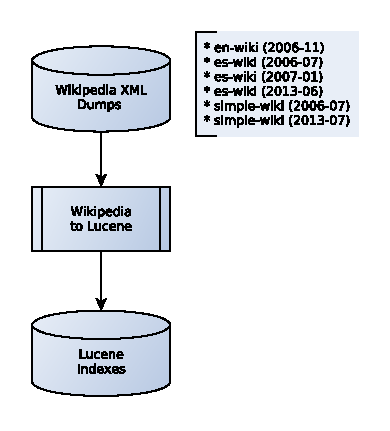
\includegraphics{graficos/LuceneIndexWriterWiki}
  \caption{Lucene Index Writer para dumps de Wikipedia}
  \label{fig:LuceneIndexWriterWiki}
\end{figure}


\subsection{Anotado de la pregunta}

El módulo original de QA-sys de procesamiento de la pregunta espera preguntas en el formato Aquaint definido por Trec, al igual que el tipo de datos esperado sobre el corpus en el paso anterior. En el procesamiento lleva a cabo las tareas descriptas de modo general en \allref{subsec:impl-pos}, \allref{subsec:impl-ner} y \allref{subsec:qtype},  utiliza como librerías de procesamiento de lenguaje el POS-Tagger, el NER-Tagger y el Question Classifier de la Universidad de Stanford, disponibles solo para inglés, descriptas en \allref{sec:stanford-both} y \allref{sec:stanford-qc} respectivamente.

En nuestra adaptación incorporamos los módulos de POS y NERC multilingües de freeling. Con respecto a la clasificación de preguntas, ya mencionamos que no existen clasificadores para español y tampoco para el portugués. Frente a esta situación podríamos haber implementado clasificadores heurísticos basados en reglas escritas a mano como en el caso del sistema estructurado (\allref{sec:qp-mitic}). Aprovechando la disponibilidad de una traducción confiable al inglés de las preguntas en archivos de datos (debido a la activación de los ejercicios cross-lingual en-es y en-pt), decidimos utilizar el clasificador de Stanford sobre la traducción inglesa de la pregunta.
Las tablas \ref{table:qc-es} y \ref{table:qc-pt} presentan la distribución de las 200 preguntas para español y para portugués según las seis clases principales del esquema de Li \& Roth. 

\begin{table}
\centering
\begin{center}
\begin{tabular}{| l | l | }
\hline
Clase & \# Preguntas  \\ \hline
HUM &  62\\ \hline
NUM &  53\\ \hline        
ENTY &  34\\ \hline
DESC &  25\\ \hline
LOC &  24\\ \hline    
ABBR &  2\\ \hline
\end{tabular}
\caption{Distribución por clases de las preguntas para el ejercicio monolingüe español}
\label{table:qc-es}
\end{center}
\end{table}



\begin{table}
\centering
\begin{center}
\begin{tabular}{| l | l | }
\hline
Clase & \# Preguntas  \\ \hline
HUM &  53\\ \hline
NUM &  52\\ \hline        
ENTY &  28\\ \hline
DESC &  30\\ \hline
LOC &  36\\ \hline    
ABBR &  1\\ \hline
\end{tabular}
\caption{Distribución por clases de las preguntas para el ejercicio monolingüe portugués}
\label{table:qc-pt}
\end{center}
\end{table}

Al finalizar este paso, las preguntas tienen asociadas su tipo, las distintas entidades nombradas, el análisis gramatical y las qwords. Dejamos la generación de queries para el paso posterior ya que así es como estaba implementado en el sistema original.

\subsection{Generación de Respuestas}
\subsubsection{Baseline}

Como baseline de desarrollo y pruebas, adaptamos los algoritmos de Qanus. En esta subsección vamos a describir esta implementación con detalle, mencionando los cambios más importantes que realizamos para adaptarla a la tarea elegida. En las siguientes comentaremos diferentes modificaciones y algoritmia agregada. El proceso de qanus para la generación de respuestas puede estructurarse así:
\begin{enumerate}
  \item Filtrado de preguntas
  \item Generación de Queries
  \item Information Retrieval
  \item Extracción y rankeo de oraciones
  \item POS tagging de las mejores oraciones
  \item Heurísticas de AR basadas en el QC
\end{enumerate}

En el primer paso, se descartan todas las preguntas cuyo tipo no sea \textit{factoid}. Esto, en principio, dejaría afuera a 32 preguntas de tipo \textit{definition} y 10 de tipo \textit{list} para el ejercicio en español (24 y 9, respectivamente, considerando solamente las que como goldstandar answer tienen datos de wikipedia) y 31 de tipo \textit{definition} y 10 de tipo \textit{list} para el portugués (18 y 8, respectivamente, considerando las de wikipedia). 

En en segundo paso, la generación de queries, el sistema baseline utiliza 2 algoritmos diferentes según el qtype inferido por el clasificador de preguntas. El primer caso es especifico para la clase fina \sq{HUM:ind} y consta de tres tipos de expresiones regulares escritas a mano y en inglés que matchean contra preguntas de la forma: \dq{Who (is|was) (the)+ NN ... NN?} (NN significa, acá, sustantivo). Por ejemplo: \dq{Who is the CEO of Microsoft?} y \dq{Who VERBO ...?}. En estos casos se extraen los sustantivos y los verbos de la pregunta para generar la query. Eliminamos estos casos ya que adaptarlos a los diferentes idiomas no escalaba para un sistema multilingüe. Por su parte, si el tipo de la pregunta no es \sq{HUM:ind}, el algoritmo general de generación de queries espera, además de la pregunta propiamente dicha, un campo asociado a la pregunta, \sq{target}, aparentemente definido en la competencia TREC para la que está escrito. 

{\color{red}Utilizamos este valor esperado para completar con el \sq{topic} del grupo de preguntas, lo cual no está permitido en las reglas originales de la competencia. }
El método default FormQuery genera una query que contiene, sin repetir, todas las palabras no-stopwords del campo target y todos los sustantivos, verbos y adjetivos de la pregunta completa según el pos tagger de stanford. Nosotros adaptamos este método para funcionar con las etiquetas de Freeling y utilizamos este mecanismo de generación de queries como baseline.

En el tercer paso, a partir de la query generada, se hace un pedido al índice lucene. En el cuarto paso, los documentos son divididos en oraciones de manera indiscriminada, es decir: las oraciones no heredan posición de acuerdo al ranking de los documentos a los que pertenecían. Las oraciones se evaluan mediante diferentes métricas contra la query generada. Los scores $coverage$, $freq$ y $prox$ están descriptos en el Apéndice \allref{sec:comparadores}. La fórmula de ponderación es la siguiente: \\

$DocScore = (0.9)*CoverageScore + (0.05)*FreqScore+ (0.05)*ProxScore;$

\medskip

En el quinto paso se seleccionan las 40 oraciones mejor rankeadas según este score y se les aplica pos tagging. 

Finalmente, el sexto paso ejecuta diferentes heurísticas de extracción de respuestas en base al tipo de pregunta generador por el clasificador en el paso anterior.
Define diferentes heurísticas para los siguientes casos: ABBR:exp, ABBR:abb, HUM:gr,
\begin{enumerate}
  \item ABBR:exp: Extrae las NER de tipo organización de la pregunta. Genera regex expandiendo la abreviación. Por ejemplo: IBM --> I.... B... M.... Para cada una de las  40 oraciones, verifica por la ocurrencia de esa regex. Devuelve la primera ocurrencia. 
  \item ABBR:abb: // Abbreviations : Contractions -> What can we do?
	\item HUM:gr || ENTY:cremat
				// HUM:gr - Human groups (companies, organisations)
			// ENTY:cremat - Entities

			// Can try to identify the subject of the question, i.e. company, university, etc
			// Heuristically, this is usually the /NN after a /WDT or /WP.

			// Tried some ideas, but gave up on them as they are not helping. One thing tried:
			// 0. Identified the "subject" of the question. For example in "what company...", the subject is "company".
			// 1. Ran a web search for candidate answer and the subject and score the number of hits matched
			// 2. Combined this with other scores like proximity etc
			// Conclusion: Helped for some queries, but when we try to query "us" and "university" for example, these
			//   are very generic terms, it didn't help.

			

			// Now we try to extract candidate answers --- these would be the proper nouns (NNP)
			// We extract them from all the ranked sentences
			// We assume consecutive NNPs are part of the same NNP.
			// i.e. Tiger/NNP Woods/NNP form one NNP
	
	
  \item HUM:
  	// All other types of HUMAN questions
			

			// Take the best ranked sentence, extract the first NNP from it and use that as the answer
  \item NUM:period
  \item NUM:count
  \item NUM:
  \item ENTY:
  \item Else
\end{enumerate}

\textbf{Adaptación inicial contra inglés}

Como las tareas cross-lingual y monolingual se cruzaban, estaban disponibles también en inglés las preguntas para nuestras tareas. 
Como paso de desarrollo, implementamos una solución sobre una wikipedia en inglés con las herramientas de procesamiento originales del baseline: StanfordNER y StanfordPOS. Lamentablemente, la tarea inglés-inglés no fue propuesta, por lo que no disponemos de las goldstandard answers como las que disponemos para español y portugués. De todos modos, realizamos experimentos sobre este sistema, utilizando la wikipedia en inglés de noviembre de 2006.

\textbf{Baseline multilingüe}

\subsubsection{Group Entity extraction}
\label{subsubsec:entidad-de-grupo}
\falta
Formas de extraer la entidad de grupo o tópico y de incorporarlo en la query.
\subsubsection{Query Generation}
\falta
Baseline de Qanus.
Resultados.
\subsubsection{Passage Extraction}
\falta
\subsubsection{Lasso Heuristics}
Métricas de medición: definición de documento relevante.
\subsubsection{Qanus baseline}
\falta
\subsubsection{Heuristic 1}
\falta
\subsubsection{Heuristic 2}
\falta
\subsubsection{Heuristic 3}
\falta
\subsubsection{Experimentación de Answer Retrieval}
\falta


\section{Evaluación}
\label{sec:eval}
\falta
\subsection{Evaluación y resultados de Clef}
\falta
Como en años anteriores, la respuesta correcta pudo estar copiada y pegada exactamente desde el documento, aún cuando sea gramaticamente incorrecta (por ejemplo: el caso de inflexión no coincide con el requerido por la pregunta). De todos modos, este año se les permitió a los sistemas usar generación de lenguaje natural para corregir inconsistencias morfosintácticas. (Por ejemplo, en alemán cambiar “dem Presidenten” por “der President” si la pregunta implica que la respuesta está en caso nominativo) y para introducir cambios gramáticos y léxicos (por ejemplo: Pregunta: ¿De qué nacionalidad es X? Respuesta: X es de Holanda => Respuesta Exacta: Holandés).


% \chapter{Implementación}
% \label{chap:implementacion}

% \section{Frameworks}

% \subsection{No funcionales}

% Para la implementación de nuestro sistema, originalmente, evaluamos la
% utilización de distintos frameworks disponibles. DeepQA, el producto
% de IBM, no es de código abierto, por lo que acerca de su
% implementación sólo sabemos lo que ventilaron en sus artículos
% técnicos. Just.ask, el sistema basado en web comparado contra
% OpenEphyra no está disponible en la web al momento de escribir este
% trabajo, mientras que OpenEphyra no funciona tal cual está dise\~nado
% originalmente (basado en web), sino que el autor sugiere unos pasos
% esotéricos para configurarlo para usar conocimiento local. Cabe
% destacar que esta falla en la funcionalidad está asociada a la que
% había encontrado [AUTOR DE PAPER EPHYRA1] en Aranea y está
% vinculado con una serie de medidas restrictivas tomadas por las
% compa\~nías de buscadores, que fueron cerrando sus accesos gratuitos
% para la comunidad de investigación bloqueando sus APIs y el acceso
% automático a sus UI. Las alternativas para el uso de buscadores,
% actualmente, se reducen a la configuración de una serie de proxies
% sobre los que rotar el acceso a la UI y así enga\~nar al detector de
% accesos automáticos -alternativa de legalidad cuestionable - o bien al 
% pago por una quota de queries por mes.
% OpenEphyra sobrevivió a Aranea porque sus responsables escribieron
% una interfaz para Bing cuando Google cerró sus puertas, mientras que
% los responsables de Aranea no lo hicieron. Finalmente, Bing también
% bloqueo el acceso automático gratuito. Notar que el mismo tipo de
% discontinuación ocurrió con el API de traducciones de Google. La
% empresa declara, explícitamente, que no está dispuesta a acceder a
% ninguna quota de acceso gratuito para la investigación académica y
% que todos sus servicios son pagos. 

% %Tanto de Aranea como de OpenEphyra podríamos llegar a tomar algunos de
% %sus componentes a la hora de construir nuestro sistema. Por el momento,
% %fueron simplemente dejados de lado.

% \bigskip

% \subsection{Qanus}

% Finalmente, un sistema que \textit{sí} estaba disponible y funcionando
% fue Qanus, que respetaba al pie de la letra su detalle técnico. Al comienzo
% del proyecto, contábamos con un corpus de datos en XML,
% lo cual coincidía, al menos en gran parte, con el input esperado de
% la implementación Qa-sys. A pesar de esto, la adaptación de los
% componentes no fue nada trivial y requirió un tiempo excesivo. En
% particular, existían dos opciones a la hora de construir un sistema
% sobre la arquitectura Qanus: dejar de lado la implementación Qa-sys e
% implementar todos los componentes de cero sobre la arquitectura, respetando las interfaces
% dadas por el framework, o adaptar el sistema funcionando para que
% trabaje sobre los nuevos datos y el nuevo entorno esperado. Frente a
% esta alternativa, se aparece claro que el framework en sí mismo no
% aporta demasiado, pues lo único que hace es atar la implementación
% final a una interfaz estructurada de tres procesos bastante sencillo.
% Además, existe un cierto grado de dependencia de la arquitectura
% hacia la implementación final, quizás no a nivel técnico, pero si
% en el modo en el que está definida la estructura. Por este motivo,
% encaramos una adaptación de Qa-sys a nuestro modelo de datos y a
% nuestros requerimientos, pero los resultados no fueron buenos en
% términos de resultados por tiempo invertido. El tiempo de aprendizaje
% del framework mismo y el tiempo requerido para adaptar las distintas
% componentes propias a las interfaces esperadas por Qanus es demasiado
% alto para la solución que brinda. Como recién mencionamos, en
% realidad, el proceso de pipeline de tres pasos no tiene tantas aristas,
% y adaptarse a un framework es mucho menos ameno que escribirlo. Este
% puede ser uno de los motivos por los cuales, como acertadamente
% se\~nalan los autores de Qanus, no existe ningún framework
% estandarizado dentro del ámbito de la investigación en QA.
% Después de la investigación inicial, podríamos concluir que
% está estandarizado, al menos a modo conceptual, la idea de que la
% resolución del problema se debe enfocar como un pipeline de al menos
% tres pasos que incluyen:
% \begin{itemize}
% \item el preprocesamiento de la base de conocimiento,
% \item el preprocesamiento de la pregunta,
% \item el retorno de la respuesta a partir de los resultados de los dos pasos anteriores. 
% \end{itemize}
% Como último comentario al respecto, el modelo de Qanus resultaba poco atractivo
%  a la hora de incorporar procesamiento en varios idiomas: el mejor approach
% utilizando esta arquitectura era implementar dos sistemas basados en
% Qanus paralelos y utilizar uno u otro de acuerdo con el resultado de
% una detección inicial. 

% \bigskip

% Si bien el modelo de Qanus fue, por los motivos recién expuestos,
% dejado de lado, debemos destacar una serie de puntos en los que fue
% útil.

% En primer lugar, uno de los objetivos de Qanus es facilitar el ingreso
% al área del QA de nuevos investigadores. Creemos que esto está
% logrado perfectamente: el código es muy sencillo y claro y lo mismo
% ocurre con la documentación, lo que hace de Qanus un proyecto muy
% útil desde una perspectiva pedagógica o educativa, más allá de
% que sea esta misma simpleza la que más adelante atente contra la
% usabilidad. El modelo de pipeline, que es el enfoque teórico usual al
% problema, y los distintos componentes y usos típicos de estos
% componentes en los distintos pasos del pipeline se realizan linealmente
% en la implementación de Qanus y Qa-sys. En particular, la similaridad
% entre la descripción del código de IBM (DeepQA y Watson) y el
% enfoque con el que Qanus ataca el mismo problema salta a la vista,
% considerando la diferencia de escalas. 

% En segundo lugar, en el plano de la investigación del estado de arte
% de los sistemas de QA disponibles creemos que el intento con Qanus
% redundó en un cierto escepticismo sobre la posibilidad de resolver
% nuestro problema utilizando herramientas disponibles de gran escala. La
% conclusión es análoga a la que tuvo el equipo de IBM al intentar
% usar OpenEphyra y PIQUANT: el tiempo de customización y adaptación
% de los framework a nuestro problema puntual es demasiado alto en
% comparación con el tiempo necesario para construir una nueva
% arquitectura que cumpla los mismos requisitos. 

% Por último, en un nivel técnico, Qanus nos resultó de utilidad para
% construir nuestro modelo final pues reutilizamos varios de los
% componentes de Qa-sys: En primer lugar, recuperamos el POS tagger, el
% NER tagger y el Question Classiffier (QC) de Stanford, que son las
% librerías principales con las que Qa-sys encara el procesamiento
% lingüístico de la pregunta y parte del proceso de generación de
% respuestas. Todas estas herramientas están disponibles en la web por
% otros medios, pero algunas -principalmente el QC- requieren un cierto
% tiempo de configuración inicial que los autores de Qanus ya habían
% resuelto. Es decir, reutilizamos, además de estos módulos externos,
% bastante de la configuración y las APIs de acceso a estos módulos
% escritos por los singapurenses. Estas herramientas funcionan bien
% sólo para inputs en inglés. Las adaptaciones que hicimos las
% veremos más abajo. Por otro lado, incorporamos casi sin
% modificaciones algunas métricas de distancia entre pasajes que Qa-sys
% usa en el momento de la generación de la respuesta como Scorers.
% Estos son las clases: \textbf{FeatureSearchTermCoverage},
% \textbf{FeatureSearchTermFrequency}, \textbf{FeatureSearchTermProximity},
% \textbf{FeatureSearchTermSpan}. Explicaremos esta métricas en breve, dentro de nuestro
% modelo, bajo en nombre de
% {\textquotedblleft}Comparadores{\textquotedblright}. Este código
% está escrito por los autores de Qanus (es decir, no es una librería externa utilizada por ellos).


% \bigskip

% \section{Arquitectura}

% \subsection{Motivación}

% En este dise\~no respetamos el modelo típico de pipeline de tres pasos que
% abunda en la literatura científica y, por lo demás, parece el
% indicado a la hora de encarar este tipo de problemas. Un momento no-técnico
% importante a destacar es la obtención de una base de datos en
% mongodb, resultado del trabajo del proyecto MITIC, la cual cambió
% sustancialmente el enfoque anterior, basado en XMLs. 
% A partir de estos datos, fue posible delinear un esquema de entidades formal que determinó
% qué se puede responder y qué no. Como vimos, la estrategia de QA
% cuando el tipo de datos es estructurado es radicamente distinta que la
% estrategia cuando los datos son no estructurados. Qanus, por su parte,
% está orientado a un tipo de datos no estructurados: buscar documentos
% rankeados en un índice de búsqueda y rastrear en ellos pasajes
% mediante distintos métodos. Cuando la base de conocimientos consta de
% un tipo de datos estructurado (esto es, de entidades, relaciones,
% atributos de entidades) es posible delimitar una ontología más
% rígida que permita concentrarse en la interpretación de la pregunta
% hacia un lenguaje formal. El arquetipo de este enfoque puede pensarse
% como la traducción de un lenguaje de consulta humano a un lenguaje de
% consulta formal, como por ejemplo, SQL: esta estrategia de QA puede
% entenderse \ como una interfaz inteligente a una base de datos. \ En
% eje principal en este acercamiento está en el análisis
% lingüístico de la pregunta a fin de mapearla a un dominio conocido
% y, por otro lado, no es necesario hacer análisis lingüístico
% sobre el corpus de datos.


% \subsection{Base de datos de dominio cerrado}
% \subsection{Ejercicios de dominio abierto}
% \bigskip





% \subsection{No Estructurado}

% El proceso de generación de respuestas para los ejercicios de la Clef es muy distinto del anterior y puede dividirse en tres pasos principales: obtención de documentos y pasajes, ranking de pasajes y generación de respuesta. En el primer paso se accede a los índices invertido (al corpus) buscando documentos relevantes. Este paso pertenece netamente al área information retrieval. Como mencionamos al comentar Watson (en particular, ver \allref{subsec:deep-qa}), es fundamental que el resultado de este paso sea lo suficientemente amplio como para contener la respuesta pero lo suficientemente acotado como para no sobrecargar el proceso posterior de análisis lingüístico sobre los pasajes. Los documentos rankeados se dividen en pasajes. En el segundo paso, tanto los documentos como los pasajes son contrastados con distintas métricas contra los datos de la pregunta generando distintos valores para estos features. Finalmente, con esta información se procede al tercer paso, que consiste en realizar diferentes filtrados sobre los pasajes en función del tipo de respuesta esperado y en distintas formas de recopilar evidencia a favor de un pasaje o una entidad (depende el caso) para finalmente seleccionar una respuesta (o decidir que no se encontró ninguna).

% \begin{figure}[H]
%   \centering
%     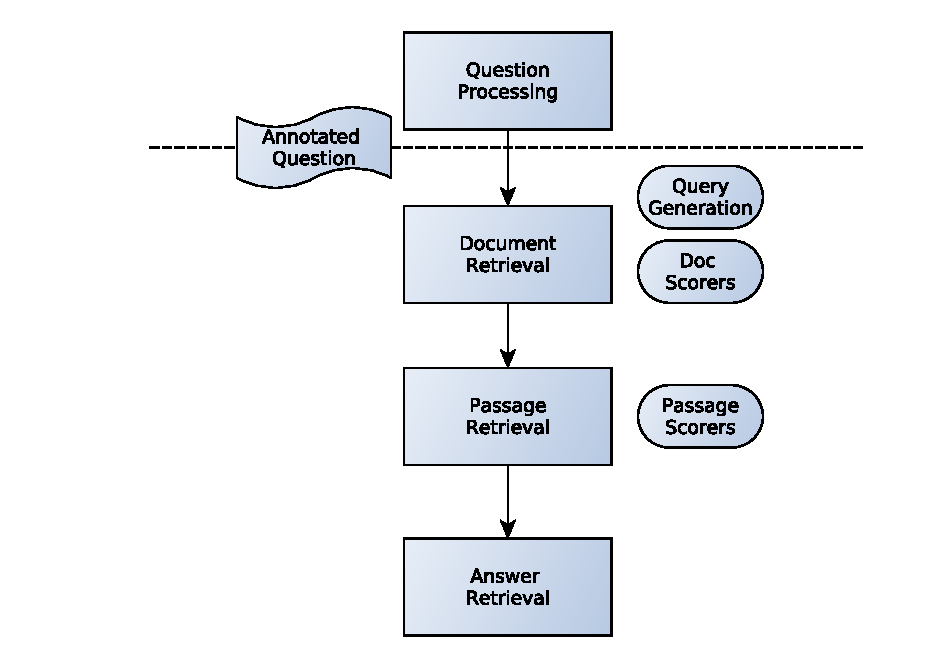
\includegraphics[scale=0.75]{graficos/AnswerRetrievalFlowWiki}
%   \caption{Flow para la Generación de Respuestas - No Estructurado}
%   \label{fig:AnswerRetrievalFlowWiki}
% \end{figure}

% \subsubsection{Documentos}
% \label{subsec:docs}
% En este punto, para una pregunta dada se dispone de la entidad del grupo de preguntas y de las distintas anotaciones hechas a la pregunta en el paso anterior (\allref{sec:qprocess}). Por su parte, los documentos en los índices invertidos poseen los campos $Id$, $Title$, y $Text$. El mecanismo de generación de queries tiene como objetivo priorizar en el ranking los documentos relacionados con el tema asociado al grupo de preguntas. Este paso es un problema de information retrieval puro: esto es, dado un pedido de información, retornar \textit{documentos relevantes}. El análisis semántico tiene peso en el paso posterior, a la hora de rankear pasajes. Por ejemplo, para el primer grupo de preguntas acerca de Harry Potter, solo se espera de este una lista de de documentos relacionados con ese mundo, en primer lugar. Por otro lado, es necesario que los principios de generación de queries no sean demasiado estrictos. Si en este punto quedan afuera muchas ocurrencias de una respuesta, entonces todo el resto del programa se ve afectado de manera irreparable. Es preferible generar documentos de más y luego filtrarlos mediante análisis lingüístico que ser demasiado estrictos y perder respuestas. 
% Para lograr esto, ponderamos los documentos en los que las entidades nombradas reconocidas lingüísticamente aparecen en el título, si se dispone de más de una entidad buscamos documentos que mencionen ambos, luego priorizamos los documentos que poseen estas entidades dentro del cuerpo y también consideramos la presencia de verbos en diferentes conjugaciones y de sustantivos que ocurren en la pregunta. Finalmente, agregamos una lista de documentos enviando la pregunta misma como una query.  

% Dado que finalmente se realizan queries simples (masivas), cabe preguntarse cual es la razón de la generación de queries y la ponderación de documentos. Esta razón es que en el proceso de ranking de pasajes y evaluación de respuesta se utilizan features basados en el score dado por lucene a los diferentes documentos. Si una mejor posición del documento contenedor del pasaje no implica que el pasaje sea correcto, si en cambio es un indicador de que dicho pasaje se encontró más cerca o más lejos del nucleo temático en el que se esperaba encontrarlo. 

% Una vez generada la lista de documentos rankeados según lucene, se procede a analizar algunos features en base a distintos scorers propios. A su vez, estos distintos valores se combinan en una evaluación general del documento, que será utilizada luego a la hora de generar una respuesta. Estas dimensiones buscan en el título y en el artículo diferente medidas sobre las entidades nombradas y sobre la pregunta completa. En concreto, se miden distancias a la entidad nombrada que identifica al grupo de preguntas (ver \allref{subsec:entidad-de-grupo}), las entidades nombradad en la pregunta misma, a la pregunta completa y la respuesta esperada data. Las medidas contra la respuesta esperada -dada por Clef- no pueden usarse para generar la respuesta, pero sí para evaluar la performance del sistema. En el siguiente cuadro se muestran las dimensiones que se consideran sobre los documentos. 

% \begin{center}
% \begin{tabular}{| l | l | l |}
% \hline
% Entidad & Campo & Comparador \\ \hline
% \multirow{6}{*}{Entidad de Grupo} & \multirow{3}{*}{Título} & Span \\ 
% & & Covr \\
% & & Freq \\ \cline{2-3}
% & \multirow{3}{*}{Texto} & Span \\ 
% & & Covr \\
% & & Freq \\ \hline
% \multirow{6}{*}{Entidades de Pregunta} & \multirow{3}{*}{Título} & Span \\ 
% & & Covr \\
% & & Freq \\ \cline{2-3}
% & \multirow{3}{*}{Texto} & Span \\ 
% & & Covr \\
% & & Freq \\ \hline
% \multirow{6}{*}{Todas las entidades} & \multirow{3}{*}{Título} & Span \\ 
% & & Covr \\
% & & Freq \\ \cline{2-3}
% & \multirow{3}{*}{Texto} & Span \\ 
% & & Covr \\
% & & Freq \\ \hline
% \multirow{6}{*}{Pregunta} & \multirow{3}{*}{Título} & Span \\ 
% & & Covr \\
% & & Freq \\ \cline{2-3}
% & \multirow{3}{*}{Texto} & Span \\ 
% & & Covr \\
% & & Freq \\ \hline
% \multirow{6}{*}{Respuesta} & \multirow{3}{*}{Título} & Span \\ 
% & & Covr \\
% & & Freq \\ \cline{2-3}
% & \multirow{3}{*}{Texto} & Span \\ 
% & & Covr \\
% & & Freq \\ \hline
% Score según índice & -- & -- \\ \hline
% \end{tabular}
% \end{center}

% Los comparadores señalados ($Freq$, $Covr$, y $Span$) se utilizan en distintos lugares de esta tesis y su funcionamiento es explicado en el apéndice \allref{sec:comparadores}. Notar que `Entidades de la pregunta' refiere tanto a aquellas reconocidas por el NER-tagger como a construcciones sustantivadas y que `Pregunta' no es la pregunta bruta sino la priorización de verbos conjugados, sustantivos, adjetivos y entidades. 

% El score general del documento es un cálculo ponderado de estas diferentes dimensiones. 

% Lucene permite especificar cuántos documentos queremos recuperar. Para evaluar la performance de este paso, utilizamos medida distintos scores en base a la respuesta dada por dada por la conferencia para el ejercicio. Es importante notar que dado que no utilizamos las imagenes de wikipedia de la primera sugerencia, es esperable que las respuesta no estén `tal cual'. 
% Evaluamos distintos mecanismos de generación de documentos, con distinta cantidad total, bajo distintas métricas. Para generar documentos, probamos la query trivial $ALL: pregunta$ (1), una un poco mejorada $ALL: entidad_de_grupo pregunta$ (2), secuencias concatenadas de queries tal como las describimos más arriba (3) y varios pedidos separados aplanados en un paso posterior (4). Para los cuatro métodos eliminamos los signos de puntuación. Para medir los resultados, utilizamos los comparadores de presencia exacta y diferentes grados de cobertura de términos (.8, .9 y 1). A su vez, evaluamos distintas imagenes de wikipedia para el español. Es total de preguntas del ejercicio, recordamos, es 200. Los resultados son los siguientes.

% \begin{center}
% \begin{tabular}{|l|l|l|l|l|l|l|}
% \hline
% Método & \# Docs & Wikipedia & Exacto & Covr 1 & Covr .9 & Covr . 8 \\ \hline

% \multirow{6}{*}{1 - Trivial} & 
% \multirow{3}{*}{100} & es - 2006 & 132 & 151 & 152 & 159 \\ 
%  &  & es - 2007 & 144 & 159 & 160 & 164 \\
%  &  & en - 2006 & x & x & x & x \\ \cline{2-7}
%  & \multirow{3}{*}{1000} & es - 2006 & 144 & 167 & 167 & 173 \\  
%  &  & es - 2007 & 159 & 177 & 177 & 180 \\
%  &  & en - 2006 & x & x & x & x \\ \hline

% \multirow{6}{*}{2 - Trivial'} & 
% \multirow{3}{*}{100} & es - 2006 & 138 & 156 & 157 & 164 \\ 
%  &  & es - 2007 & 151 & 167 & 168 & 171 \\
%  &  & en - 2006 & x & x & x & x \\ \cline{2-7}
%  & \multirow{3}{*}{1000} & es - 2006 & 147 & 168 & 168 & 174 \\ 
%  &  & es - 2007 & 163 & 178 & 178 & 181 \\
%  &  & en - 2006 & x & x & x & x \\ \hline
% hola & ey &wiki& 137 & 156 & 157 & 160  \\ \hline
% \multirow{6}{*}{3 - Inteligente} & 
% \multirow{3}{*}{100} & es - 2006 & 127 & 144 & 144 & 150 \\ 
%  &  & es - 2007 & 141 & 150 & 151 & 156 \\
%  &  & en - 2006 & x & x & x & x \\ \cline{2-7}

%  & \multirow{3}{*}{1000} & es - 2006 & 143 & 163 & 163 & 170 \\   
%  &  & es - 2007 & 158 & 175 & 175 & 179 \\
%  &  & en - 2006 & x & x & x & x \\ \hline

% \multirow{6}{*}{4 - Inteligente'} & 
% \multirow{3}{*}{100} & es - 2006 & 142 & 160 & 161 & 168 \\ 
%  &  & es - 2007 & 157 & 170 & 171 & 174  \\
%  &  & en - 2006 & x & x & x & x \\ \cline{2-7}


%  & \multirow{3}{*}{1000} & es - 2006 & 147 & 168 & 168 & 174 \\ 
%  &  & es - 2007 & x & 158 & x & x \\
%  &  & en - 2006 & x & x & x & x \\ \hline
 
% \end{tabular}
% \end{center}

% Conclusión de esto.

% \subsubsection{Pasajes}
% Este paso es análogo al anterior, pero con mayor detalle y granularidad. Cada documento generado en el paso anterior, con sus diferentes puntajes para 
% las dimensiones señaladas, se parten en pasajes u oraciones. Nuevamente, sobre estas oraciones realizamos diferentes mediciones y las combinamos generando
% un score final. En esta sección discutiremos las mediciones consideradas y los diferentes métodos de combinación de las mismas. Estos métodos de combinación generan distintos rankings de pasajes. Para evaluar estos rankings, nuevamente, utilizaremos la información disponible sobre las respuestas esperadas, buscando que la respuesta esperada se encuentre entre los $n$ pasajes mejor rankeados.
% En primer lugar, las distintos scorers implementados son los siguientes:

% \begin{center}
% \begin{tabular}{| l | l | l |}
% \hline
% Comparador & Qué & Dónde \\ \hline
% \multicolumn{3}{|c|}{Estadísticos} \\ \hline
% Freq & Pregunta & Pasaje \\ \hline
% Span & Pregunta & Pasaje \\ \hline
% Covr & Pregunta & Pasaje \\ \hline
% \#Tokens & -- & Pasaje \\ \hline
% \multicolumn{3}{|c|}{Basados en NLP} \\ \hline
% Presencia & Entidad de Grupo & Pasaje \\ \hline
% Presencia & Entidades de pregunta & Pasaje \\ \hline
% Presencia & Verbos de pregunta & Pasaje \\ \hline
% Presencia & Sustantivos de pregunta & Pasaje \\ \hline
% \multicolumn{3}{|c|}{Para evaluación} \\ \hline
% Freq & Respuesta & Pasaje \\ \hline
% Span & Respuesta & Pasaje \\ \hline
% Covr & Respuesta & Pasaje \\ \hline
% \end{tabular}
% \end{center}

% A estos Scorers se le suman los scores del documento asociado al pasaje (ver \allref{subsec:docs}). 
% Sobre estas dimensiones disponibles, intentamos las siguientes combinaciones de priorización:

% \begin{center}
% \begin{tabular}{|l|l|l|}
% \hline
% \#& Nombre & Fórmula \\ \hline
% 1& Simple & $2+2=4$ \\ \hline
% 2& Respuesta & $2+2=4$ \\ \hline
% 3& Compleja & $2+2=4$ \\ \hline
% \end{tabular}
% \end{center}

% Y consideramos la ocurrencia de respuestas, de la misma manera que en el apartado anterior (Match Exacto y tres medidas de covertura de tokens: 1, .9 y .8), 
% sobre los primeros $n$ pasajes, con $n$ = 1, 5, 10, 20, 50 y 100.

% \begin{center}
% \begin{tabular}{|l|l|l|l|l|l|}
% \hline
% Fórmula & \#Docs & Exacto & Covr 1 & Covr .9 & Covr . 8 \\ \hline
% \multirow{6}{*}{1} & 1 & x & x & x & x \\  \cline{2-6}
%  & 5 & x & x & x & x \\ \cline{2-6}
%  & 10 & x & x & x & x \\ \cline{2-6}
%  & 20 & x & x & x & x \\ \cline{2-6}
%  & 50 & x & x & x & x \\ \cline{2-6}
%  & 100 & x & x & x & x \\ \hline
% \end{tabular}
% \end{center}


% \subsubsection{Respuestas}





% \begin{figure}
%   \centering
%     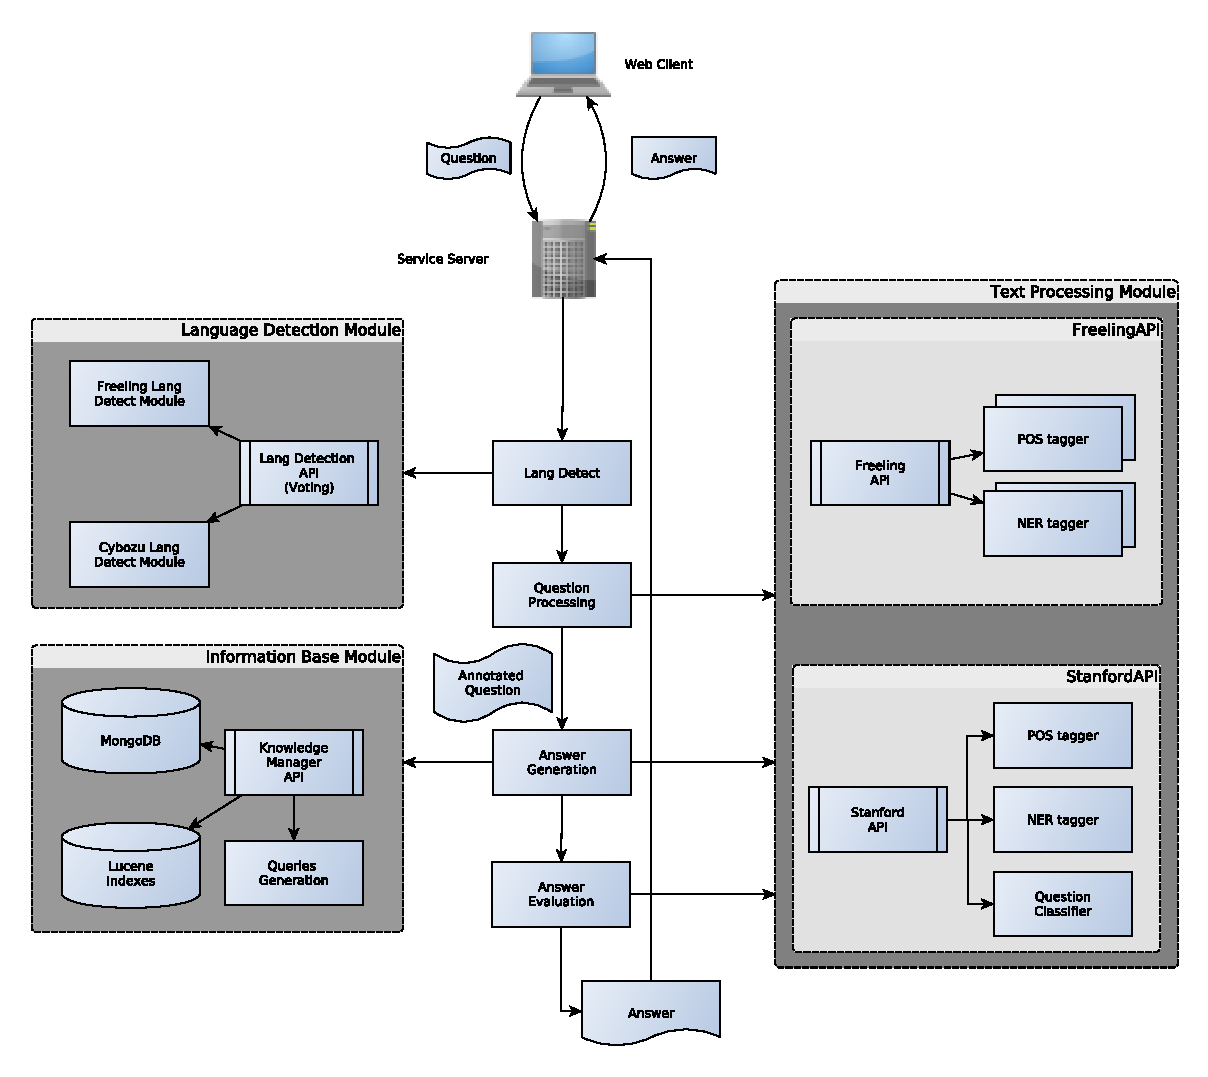
\includegraphics[scale=0.86]{graficos/Architecture}
%   \caption{Arquitectura}
%   \label{fig:Architecture}
% \end{figure}

% %\end{document}
